%\documentclass[10pt,twocolumn,journal]{IEEEtran}
%\documentclass[12pt,draftclsnofoot,onecolumn,journal]{IEEEtran}
\documentclass[10pt, conference]{IEEEtran}
\usepackage[english]{babel}
\usepackage{url}
\usepackage{cite}
%\usepackage[noadjust]{cite}
\usepackage{epsf}
\usepackage{amssymb,amsmath,amsfonts}
\usepackage{array}
\usepackage{graphics}
\usepackage{graphicx}
\usepackage{cleveref}
\usepackage{theorem}
\usepackage{algorithm}
\usepackage{algorithmic}
\usepackage{caption}
\usepackage[table]{xcolor}
%\usepackage{subcaption}
\usepackage{soul}
\usepackage{subfig}
\usepackage{minted}
\usepackage{adjustbox}
%\usepackage{color}
%\usepackage[symbol]{footmisc}
\usepackage[para]{footmisc}
%\usepackage{changes}
\usepackage[final]{changes}
%\usepackage{lineno}
%\linenumbers
\renewcommand{\thefootnote}{\fnsymbol{footnote}}
\newcommand{\smartparagraph}[1]{\vspace{.05in}\noindent\textbf{#1}}
\PassOptionsToPackage{bookmarks=false}{hyperref}

\pagestyle{empty}

%\def\symbolfootnote[#1]#2{\begingroup
%\def\thefootnote{\fnsymbol{footnote}}
%\footnote[#1]{#2}\endgroup}

%\IEEEoverridecommandlockouts
%\IEEEpubid{\makebox[\columnwidth]{978-1-7281-5684-2/20/\$31.00~\copyright{}2020 IEEE \hfill} \hspace{\columnsep}\makebox[\columnwidth]{ }}

\begin{document}

\title{Field trial of programmable L3 VPN service deployment using SDN-Based Multi-domain Service Provisioning over IP/Optical networks}

\author{
\IEEEauthorblockN{Samier Barguil\IEEEauthorrefmark{1}, Victor Lopez\IEEEauthorrefmark{2}, Cristyan Manta-Caro\IEEEauthorrefmark{4}, Arturo Mayoral Lopez De Lerma\IEEEauthorrefmark{2},\\
Oscar Gonzalez De Dios\IEEEauthorrefmark{2}, Edward Echeverry\IEEEauthorrefmark{3}, Juan Pedro Fernandez-Palacios\IEEEauthorrefmark{2}, Janne Karvonen\IEEEauthorrefmark{5},\\
Jutta Kemppainen\IEEEauthorrefmark{5}, Natalia Maya\IEEEauthorrefmark{5}, and Ricard Vilalta\IEEEauthorrefmark{6}}
\IEEEauthorblockA{
\IEEEauthorrefmark{1}Universidad Autonoma de Madrid, Madrid, Spain\\
\IEEEauthorrefmark{2}Telefonica I+D, Ronda de la Comunicacion, Madrid, Spain \\
\IEEEauthorrefmark{3}Telefonica Movistar, Transversal 60 No 114ª -55. Bogotá, Colombia\\
\IEEEauthorrefmark{4}Wipro Technologies Ltd., Doddakannelli, Sarjapur Road
Bengaluru - 560 035, India\\
\IEEEauthorrefmark{5}Infinera Corporation, 140 Caspian Court, Sunnyvale, CA 94089, USA\\
\IEEEauthorrefmark{6}Centre Tecnol\`{o}gic de Telecomunicacions de Catalunya (CTTC/CERCA), Castelldefels, Spain}}

\maketitle

\begin{abstract}
Network operators can not change their footprint to upgrade the entire Network to support SDN from scratch. \replaced{Hence,}{This why} network operators adapt\added{ed} the original SDN concept into a hybrid SDN approach to have a pragmatic, evolutionary, and economically viable solution. This paper tests an SDN architecture based on a hierarchical structure of a Software-Defined Transport Networking (SDTN) controller, which deals with the end-to-end service provision and topology collection on top of a set of SDN controllers for each technological domain. The authors demonstrate L3/L2 VPN service deployment using an underlay multi-domain IP/Optical networks in a field trial. The approach allows a service provider to migrate brownfield scenarios into SDN domains using programmatic interfaces.

\end{abstract}

\section{Introduction}
Software-Defined Networking (SDN) has emerged as the new reference paradigm to promote network automation and programmability. It has promoted the idea of a radical transformation in all aspects of the: service delivery, network, and traffic management; because end-to-end automatic service provision, automated monitoring, fast issue detection, and event-based decision taking are mandatory functionalities to offer a high-quality customer experience \cite{ordonez2017network}.

Conceptually, SDN allows a full decoupling between control and forwarding plane on Physical Network Functions (PNFs). 
This concept allows the centralization of complex processing tasks and enables integrating white boxes (i.e., smaller equipment, high port density, low processing capacity, \replaced{made}{facts} with generic hardware, and lower production cost) in the network access layers. However, this promise is still not a reality on the service provider networks. Although the term SDN seems new, it has already been more than twelve (12) years since a Stanford team defined OpenFlow and founded NICIRA (NICIRA was the first company to develop a commercial SDN controller (NOX)). Nowadays, despite millionaire investments and several SDN controller solutions available \cite{medved2014opendaylight,berde2014onos} on the market, almost no service provider has a full operative SDN network controller deployed. Some of the main barriers found by service providers until now are:

\begin{itemize}
    \item There are still many dependencies on manually executing tasks.
    \item Network control tasks can not be fully centralized.
    \item The stack of protocols deployed in the network is very complicated.  The knowledge that network operators require to solve problems continues to be very specific.
    \item Confidence in automation solutions is not very high.
    \item Many networks have grown via company acquisitions. In many cases internally they operate as independent carriers. 
    \item Standardization is not complete, generating a lack of full interoperability between vendors.
\end{itemize}

Several new approaches have been gradually released in recent years to adopt SDN as a hybrid solution in brownfield scenarios. Some of the most promising methods were defined using agile methodologies, as software development and IT operations (DevOps) solutions \cite{choi2018agile}. 
These agile methodologies usually take a small network task and solve it using a programmatic approach. It allows the simple and more frequent integration of new functionalities. Network provisioning is one of the recurrent tasks selected for agile automation; because it is a diary job that includes the usage of well-defined templates to deploy MPLS-based services on the network.

The Layer 3 Virtual Private Network (VPN) service defined in RFC 4364 \cite{rfc4364} provides a multi-point, routed service to a customer over an IP/MPLS core. L3VPNs are widely used in carrier-grade networks to deploy 3G/4G, fixed, and enterprise services. Traffic policies can be applied in these services to reuse the same transport network, and it also makes it feasible to combine access technologies over an MPLS core. On the other hand, L2 services belong to the class of IP virtual leased line (VLL) services or virtual private LAN (VPLS) services \cite{andersson2006framework}, which are a fundamental part of the service portfolio offered by service providers. 

This work proves the viability of the implementations of programmable network interfaces for the deployment of L2/L3 services in IP over optical networks using common standard models and protocols. A field trial including multiple network controllers (two for IP/MPLS and two for DWDM) and a real-commercial-multivendor-operative network was installed by Telefonica in their premises in Colombia to validate the concept.

The paper is structured as follows: \Cref{sec:soa} provides a review of the State of the Art both on the provisioning of automated L2/L3 VPN services. \Cref{section:arq} describes the SDN reference architecture and details the principles of the network programmability, including concepts of YANG and used protocols. Then, Section \ref{section:trial} details the test architecture, including commercial network controllers and the results obtained in this implementation. Finally, conclusions and perspectives are drawn in \Cref{section:conclusions}.    

\added{
The list of abbreviations and its definition is defined in \cref{tab:abbreviations}.}

\begin{table}[htb!]
\caption{List of abbreviations used across the document}
\label{tab:abbreviations}
\begin{tabular}{|l|l|}
\hline
Abbreviation & \multicolumn{1}{c|}{Definition}              \\ \hline
API          & Application programming interface            \\ \hline
BGP          & Border Gateway Protocol                      \\ \hline
BGP-LS       & Border Gateway Protocol Link-State            \\ \hline
BSS          & Business Support Systems                     \\ \hline
CE           & Customer Edge                                \\ \hline
CRUD         & Create, Read, Update and Delete              \\ \hline
DWDM         & Dense Wavelength Division Multiplexing       \\ \hline
GMPLS        & General Multi-Protocol Label Switching       \\ \hline
GUI          & Graphical user interface                     \\ \hline
IETF         & Internet Engineering Task Force              \\ \hline
IGP          & Interior Gateway Protocol                    \\ \hline
IP           & Internet Protocol                            \\ \hline
L2           & Layer-2                                      \\ \hline
L2SM         & L2VPN Service Model                          \\ \hline
L2SM         & L2VPN Service Model                          \\ \hline
L2NM         & L2VPN Network Model                          \\ \hline
L3           & Layer-3                                      \\ \hline
L3SM         & L3VPN Service Model                          \\ \hline
L3NM         & L3VPN Network Model                          \\ \hline
LAG          & Link aggregation group                       \\ \hline
LDP          & Label Distribution Protocol                  \\ \hline
MPLS         & Multiprotocol Label Switching                \\ \hline
NBI          & Northbound interface                         \\ \hline
ONF          & Open Networking Foundation                   \\ \hline
OSS          & Operation Support Systems                    \\ \hline
PCE          & Path Computation Element                     \\ \hline
PE           & Provider Edge                                \\ \hline
QoS          & Quality of service                           \\ \hline
RD           & Route Distinguisher                          \\ \hline
RPC          & Remote Procedure Call                        \\ \hline
RT           & Route Target                                 \\ \hline
SBI          & South Bound Interface                        \\ \hline
SDN          & Software Defined Network                     \\ \hline
SDNc         & Software Defined Network Controller          \\ \hline
SDTN         & Software Defined Transport Network           \\ \hline
TAPI         & Transport API                                \\ \hline
URI          & Uniform resource identifier                  \\ \hline
VPN          & Virtual Private Network                      \\ \hline
VRF          & Virtual Routing and Forwarding               \\ \hline
YANG         & Yet Another Next Generation                   \\ \hline
\end{tabular}
\end{table}

\section{State of the Art}
\label{sec:soa}

The IP service models are YANG modules defined to support the creation, deletion, and retrieval of L3/L2VPN services and the IP/MPLS network topology collection. The models used in this work are abstract models that technologically describe the network requirements and are RFCs or working-group-drafts inside the IETF.

\subsubsection{L3VPN Service Model (L3SM)}
\label{section:l3nm}
Multi-Protocol Label Switching (MPLS) Virtual Private Networks (VPNs) have seen an unparalleled increasing adoption during the last years. Although their flexibility as transport technology and their effectiveness for traffic engineering are well recognized, VPNs are hard to set up, operate, and manage, due to the complexity of the network, the protocols involved, and possible multi-vendor parameter discrepancies.

Some service models have been defined and standardized until now to support the L3VPN creation. L3SM \cite{rfc8299} is a Customer Service Model that describes an L3VPN service's configuration parameters based on customer requirements. The L3SM model keeps some commercial customer information as the "customer-site-location". This model provides an abstracted view of the Layer 3 IP VPN service configuration components. However, it is mainly focused on \replaced{the provider edge (PE)}{BGP PE-based} VPNs and doesn't have specific parameters to configure the different network elements in multi-vendor scenarios nor has the possibility to bind the services with specific transport options inside the MPLS network.  

L3NM \cite{voyer2019internet} is a complementary Network Model of the L3SM. It differs from the L3SM because it is entirely network-centric and groups all the provider edge routers (PE) configurable parameters. Network controllers can expose the L3NM to manage and control the VPN Service configuration in multi-domain scenarios. It contains valuable information to operate the service, such as each network element's identifier in the IP/MPLS domain (NE-ID) and the interface identifier of each customer access. It includes resources such as Route Targets (RTs) and Route Distinguishers (RDs).

L3NM is populated based on the services request (f.i. L3SM query) and an \replaced{SDNc}{SDN controller} includes network-specific information in the message sent to the domain controllers like transport LSP binding, routing profiles, or encryption profile. It assigns logical resources such as route targets or route distinguishers to keep the data synchronized between domains. \Cref{FIG:l3nm} shows the structure of the L3NM YANG data model, where the main container (VPN Service) is used to group the information of the VPN-Node (VRFs) and the VPN-Network Accesses (Interfaces).

\begin{figure}
	\centering
	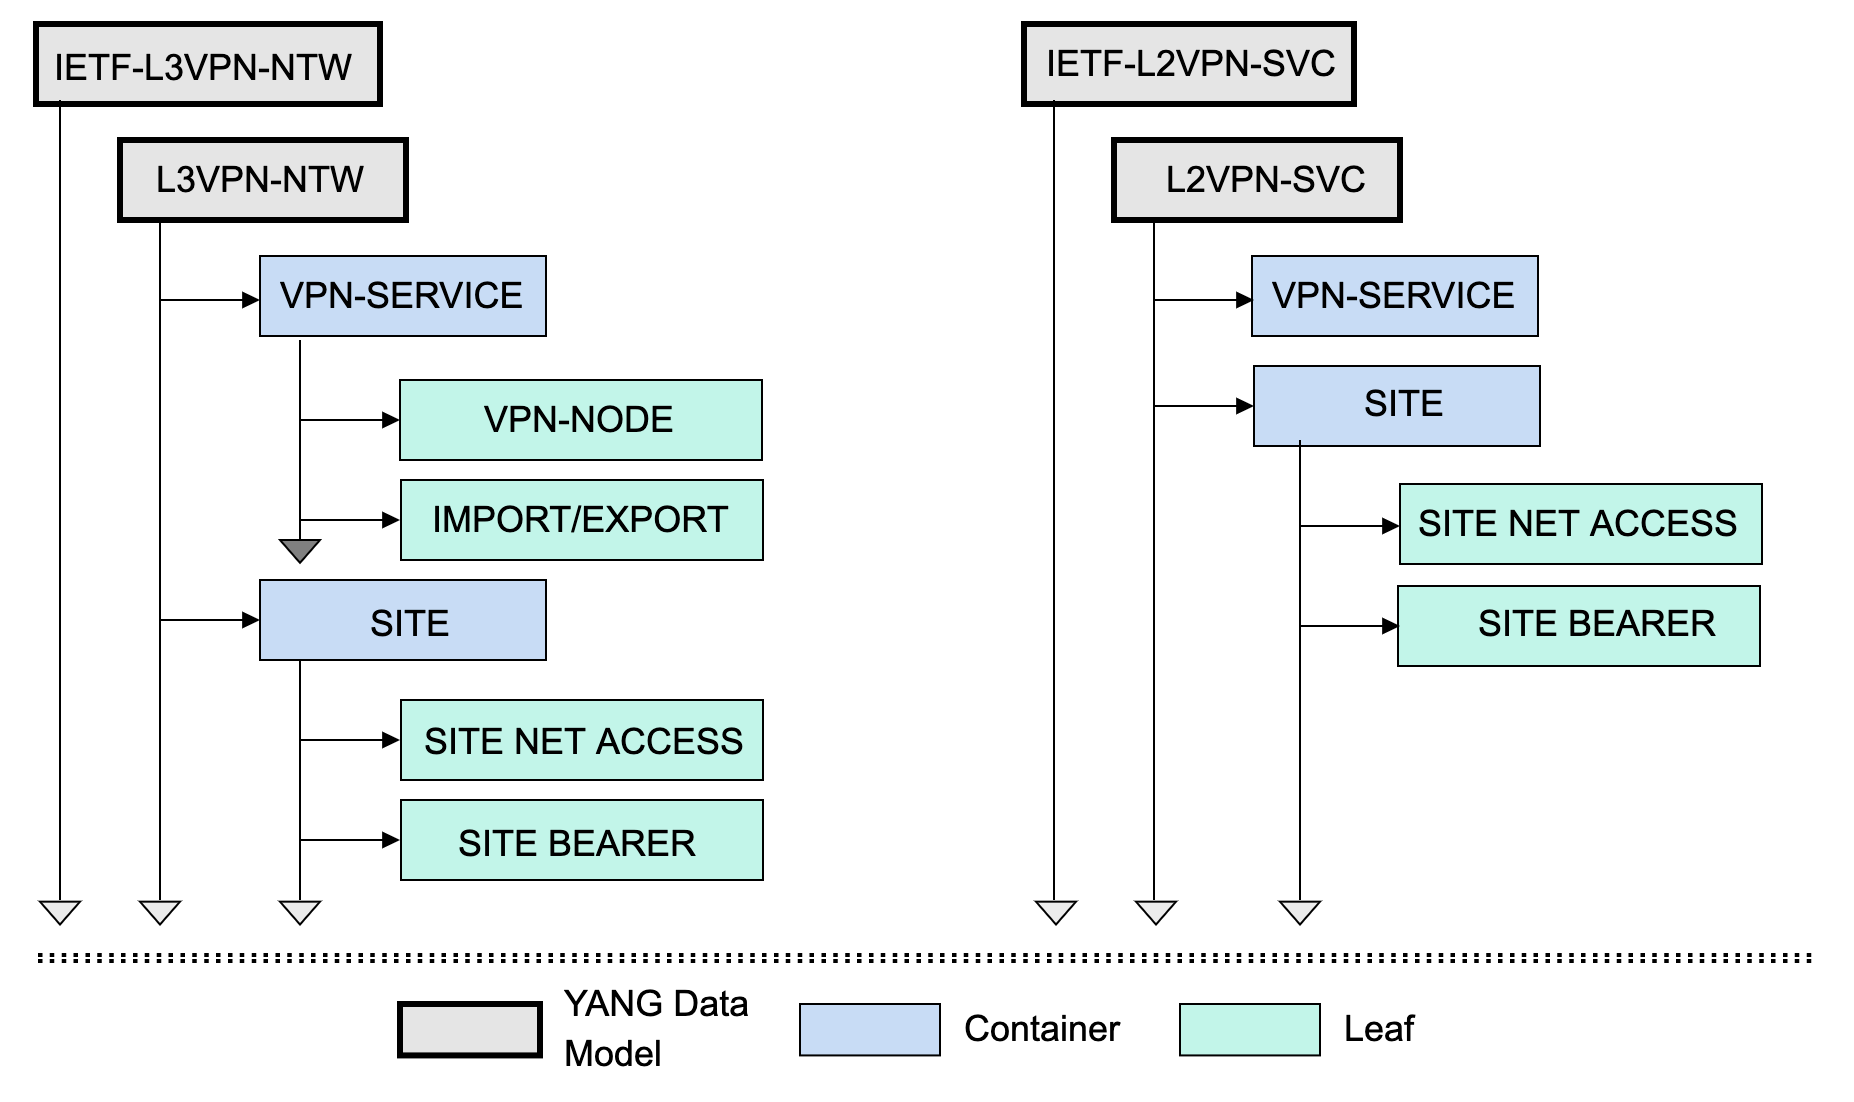
\includegraphics[width=\linewidth]{figs/diagram-10.png}
	\caption{L2NM and L3 Data models structures. The hierarchy represents a container in the YANG model. The  lines represents cross references between the containers.}
	\label{FIG:l3nm} 
\end{figure}

\subsubsection{L2VPN Service Model (L2SM)}
\label{section:l2nm}

Similarly, the IETF has standardized YANG models for the L3VPNs; there is already a standard for the L2 services. The model is named L2SM \cite{wen2018yang}. 

The L2SM is a customer-centric model; It has two main sets of parameters, the VPN Service and the site information. The \cref{FIG:l3nm} depicts the main components of the L3NM and the L2SM as a tree structure. The VPN service contains all the technological parameters of the services that are going to be deployed, for example, service type or service topology. The ``site'' includes all the customer information, like the ``customer-location'' and the access parameters between the Customer-Edge (CE) and the Provider-Edge (PE).

This model lacks some specific network parameters; those need to be stored or derived by the network controller to deploy the network device's configuration. For futures implementations, additional work to complement the current standard can be proposed.  

\section{SDN Architecture}
\label{section:arq}
\begin{figure*}[htp]
	\centering
	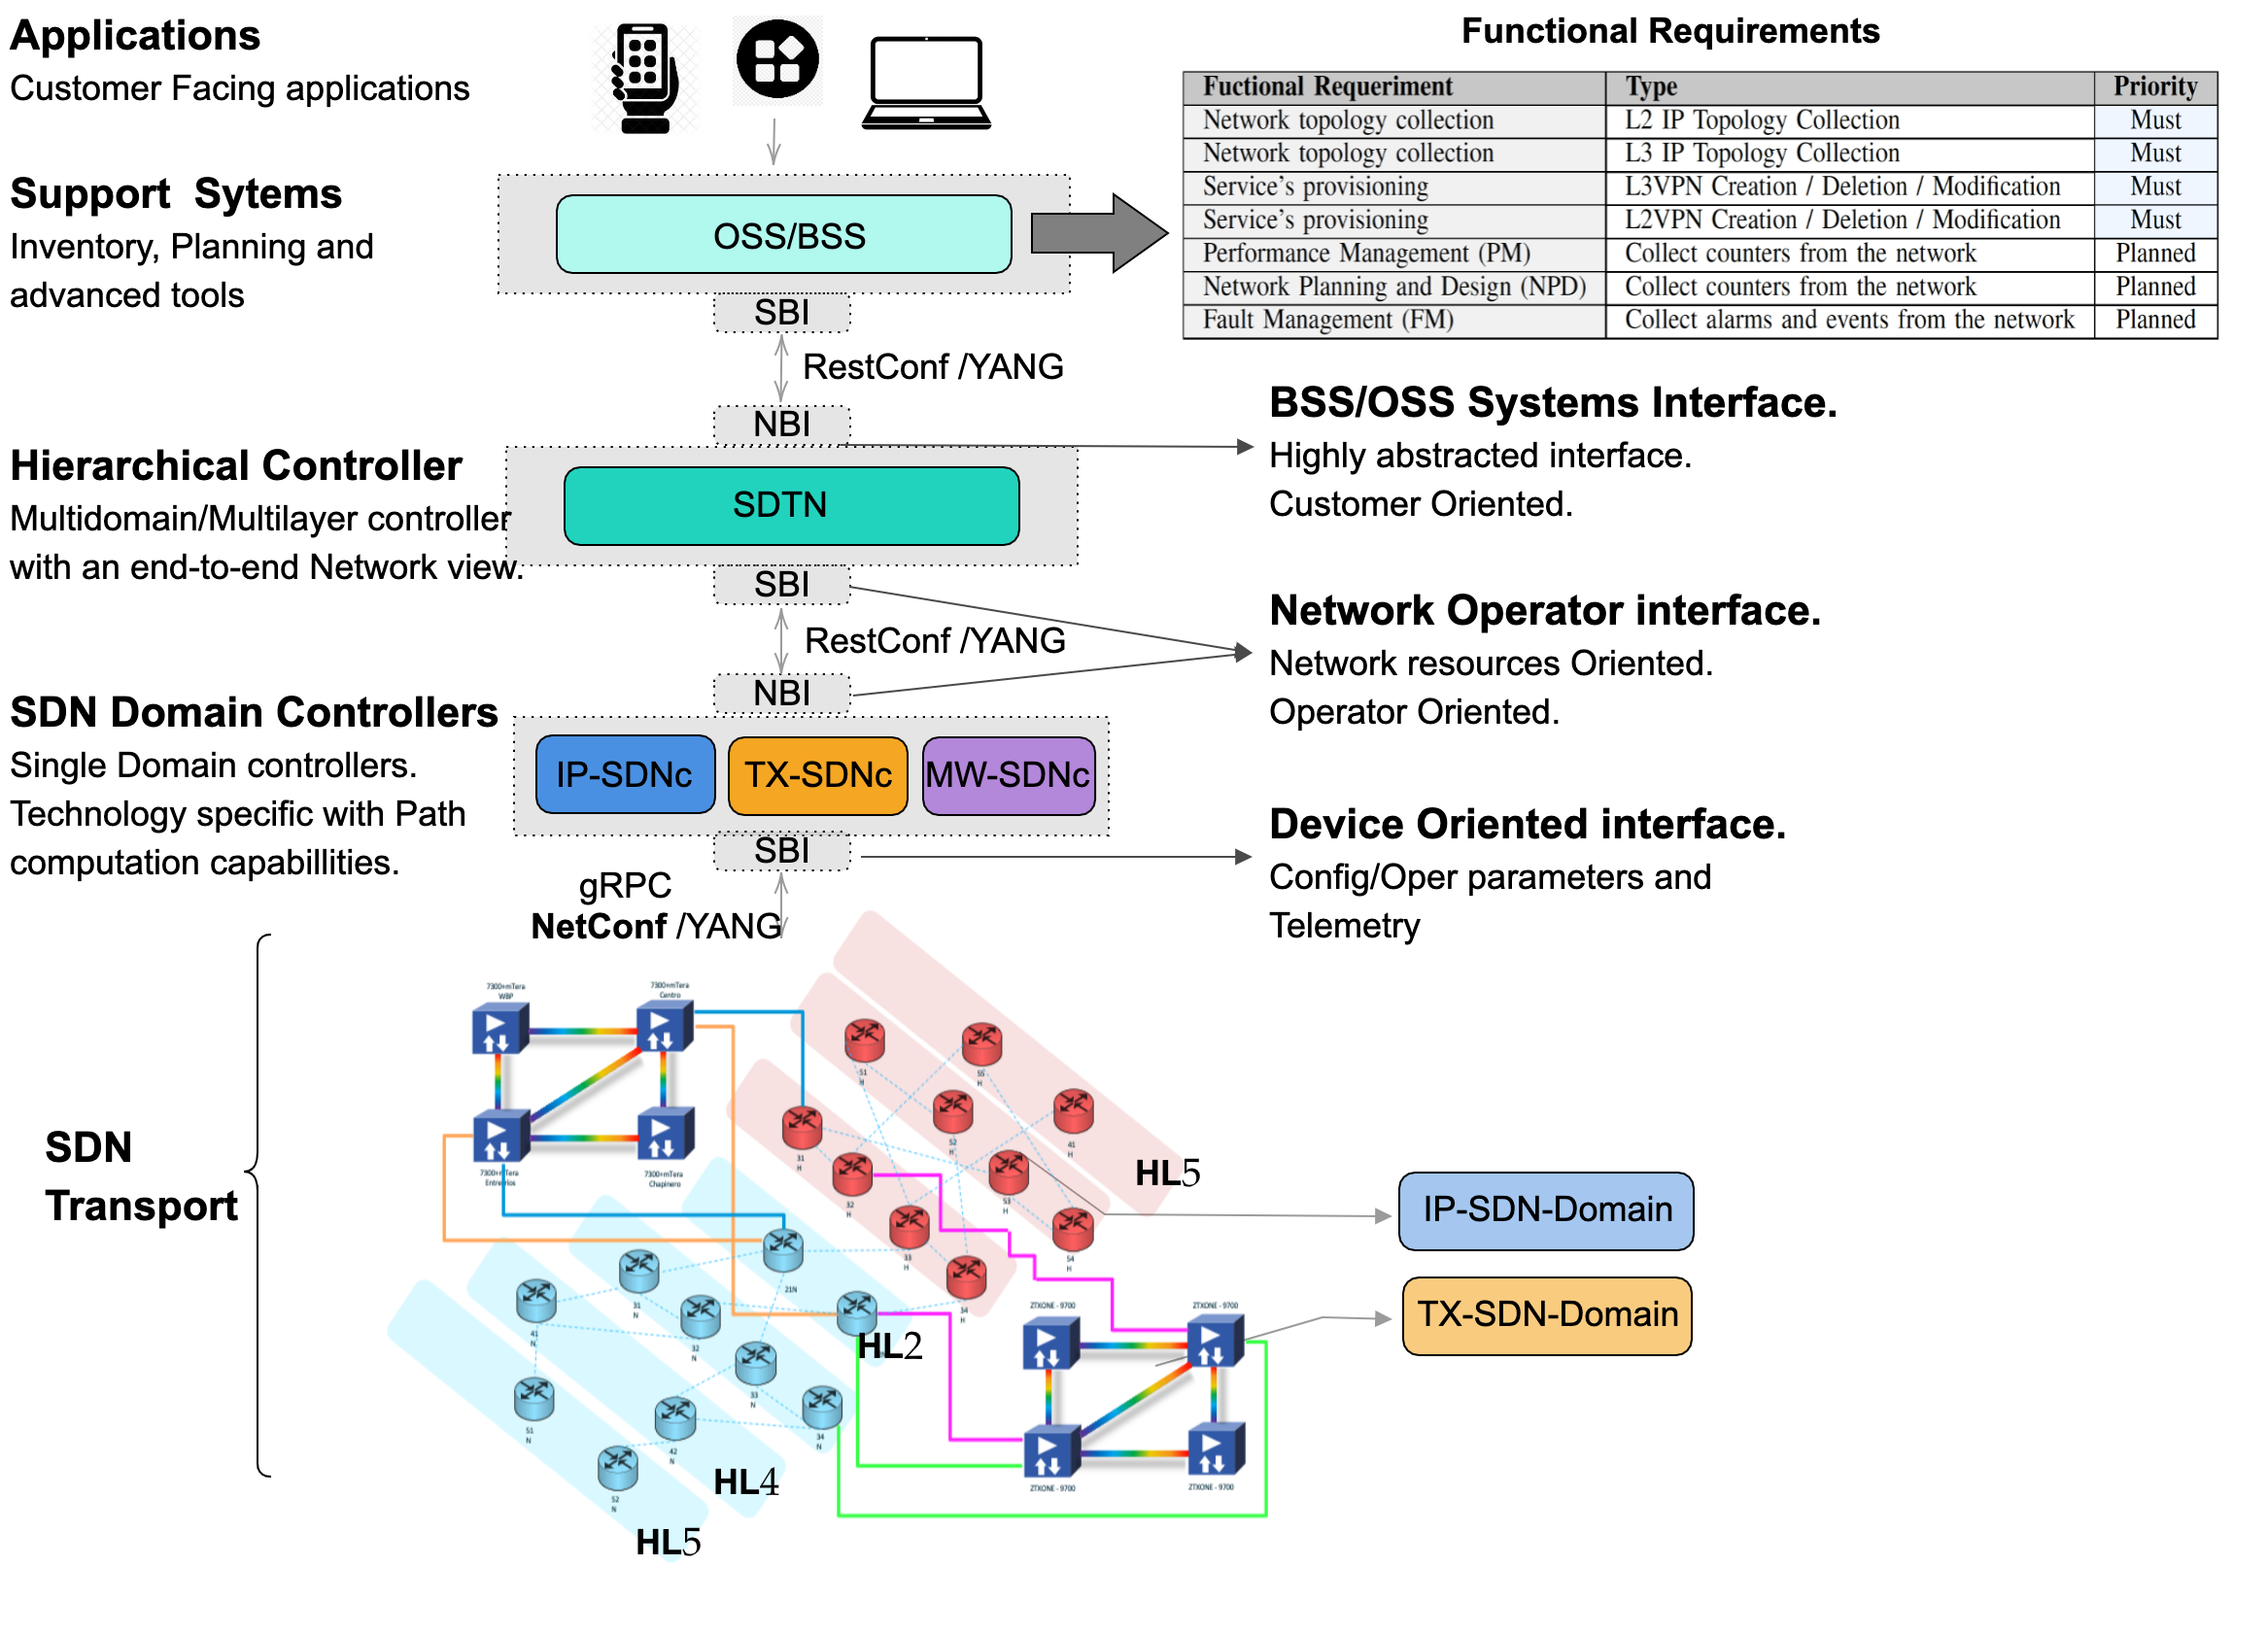
\includegraphics[width=\linewidth]{figs/diagram-1.png}
	\caption{i\uppercase{FUSION}\cite{contreras2019ifusion} architecture has two control layers. The first one having the SDTN controller with the end-to-end view of the network. Second control layer includes the SDN Domain controllers. Those controllers interact with the network devices (Fusion Network). The set of use cases Tested in the POC are listed.}
	\label{FIG:1}
\end{figure*}

i\uppercase{FUSION} is a reference model architecture defined by Telefonica to reinforce the network automation and programmability in a service provider environment. i\uppercase{FUSION} is hierarchical, with specific domain controllers per technological domain (IP/MPLS, microwave, optical)
and a hierarchical controller to provide real-time control of multi-layer and multi-domain transport network resources. The i\uppercase{FUSION} main principles include the use of: (1) Standard interfaces based on \uppercase{RESTconf/YANG} \cite{bierman2017restconf} for the communication between controllers and \uppercase{NETCONF/YANG} \cite{enns2011network} to configure the network elements; (2) YANG data models based on latest developments in the standards-development organizations (SDOs): \uppercase{IETF}, \uppercase{ONF} and OpenConfig.


The main elements of the SDN i\uppercase{FUSION} architecture are the following:

\begin{itemize}

\item \textbf{SDN Domain}: It is a set of network elements under the supervision of the same SDN Controller. There are several possible levels in the decoupling of control and data planes. The preferred level of decoupling depends on the network technology. For example, network element runs the distributed protocols (e.g. IS-IS TE, RSVP-TE) in MPLS, and the controller only needs to configure it.

\item \textbf{SDN Domain Controller (SDNc)}: This element is in charge of a set of network elements. It has standard southbound interfaces that depend on the technology, but not in the equipment vendor, to communicate with the network elements. It also has a northbound interface to communicate with the \replaced{SDTN Controller}{SDTN Orchestrator}.\added{For some use cases, like performance management, the authors initially identified the necessity to connect the OSS layer with the SDNc directly.}

\item \textbf{Software Defined Transport Network (SDTN) Controller}: In case several SDN Domains are needed, the \replaced{SDTN Controller}{SDN Transport Controller (SDTN}) is in charge of providing\added{/composing} services through several domains. 

\end{itemize}

The i\uppercase{FUSION} architecture was designed as a hierarchical model where a dedicated SDN Domain controller controls each network segment. Due to its complexity, the transport network is divided into three main technology domains: IP, Optical for transmission, and Microwave.  The proposed architecture can be shown in terms of components and relationships among them, as depicted in \cref{FIG:1}. 

The SDTN Controller is responsible to orchestrate the respective SDNcs within the transport segment (IP, Optical and MW) through the Domain Controllers'~NBI, providing an end-to-end transport network vision. The SDTN Controller aggregates demands from the management and services layer exposing a unified NBI which should provide resource configuration abstraction and technology agnostic service definition. 

\subsection {IP Domain}
\label{section:ip}
Traditionally IP networks are deployed following a regional model mixing equipment from different vendors. The IP boxes are interoperable at both data and control plane levels (e.g., routing protocols such as IS-IS, OSPF, or BGP). Due to scalability and resiliency reasons, the IP administrators divide the whole network into IP domains, so the routing and control protocols are the same in an administrative area.

The goal SDN solution for the IP segment is composed of a single IP \replaced{SDNc}{SDN controller}, whose goal is to configure all the IP network elements. The target SBI for vendor-agnostic device configuration shall be compliant with NETCONF standard protocol. \added{OpenConfig started as a collaborative work between Google, some vendors and Service Providers, and now it is an industrial reference for device-specific configuration purposes. The philosophy behind OpenConfig is to add functionality to the device models based on the operator’s needs to avoid complex models which can not be implemented in real networks.} Due to its maturity level, the set of device configuration data models are the ones defined used in i\uppercase{FUSION} are OpenConfig.

It is expected that the IP \replaced{SDNc}{SDN controller} will assume the control/management of:
\begin{itemize}
\item Device configuration of interfaces (VLANs) and routing protocols (BGP, ISIS, …)
\item Traffic Engineering of MPLS tunnels (LSPs). 
\item Overlay networks services (L2/L3 VPNs) device configuration (VRFs,\dots)
\end{itemize}

The IP SDNc will be the main entry point to the network elements, to avoid overloading the elements with external requests and providing a  full and coherent network view. The NBI of the controller in i\uppercase{FUSION} follows IETF YANG models and they are implemented on RESTCONF with JSON encoding. \added{The IETF YANG for the NBI  was done based on the support of the supplier to the models. The IETF adoption is wider than any other alternative for the NBI.}

\subsection{Optical domain}
\label{section:dwdm}
Optical transport networks from different system vendors are deployed on a regional basis, either for technology redundancy, due to different optical performance requirements (metro vs. long-haul), or simply for commercial reasons. 

Without line-side interoperability of the different optical transceivers and Reconfigurable Optical Add-Drop Multiplexers (ROADMs), there is not a competitive advantage on a uniform configuration interface of the optical devices, since they cannot neither be mixed in a multi-vendor scenario, due to the fact that both line systems and transceivers must be from the same vendor.

With this in mind, in the short term, Optical SDNc are expected to provide network programmability and interoperability towards upper layers (multi-layer) and between vendors (multi-domain, multi-vendor) through the support of standard NBIs (i.e. coordination will be provided by upper layer hierarchical SDTN \added{Controller}). This short term approach will enable the setup and tear down of connections in optical channels (OCh and ODU layers), the discovery of the network resources to compose a layered uniform view based on the OTN hierarchy, and the monitoring of the optical network in a vendor agnostic fashion thanks to the utilization of ONF Transport API (T-API) 2.1 \cite{lopez2016transport}, having been experimented in several proof of concepts \cite{mayoral2016first}. Please note, that in this transport domain, T-API + RESTCONF is also proposed to be the NBI of the hierarchical SDTN Controller towards Service B/OSS layers.

In the medium and long term, the direct programmability of the components can have interest in Point-To-Point, Metro and Regional scenarios, where disaggregation of optical transceivers and line side components can play an important role. In this line, OpenROADM \cite{oda2016learning} and OpenConfig projects have already defined device configuration models for transponders and open line systems. 

\subsection{Integration of SDTN \added{Controller} in the overall operator’s systems architecture}
\label{section:sdtn}
One of the main reasons for deploying an SDTN Controller is service automation. It facilitates that manual services and network configurations become automated and available through its NBIs, enabling the network automation progressively. As the main design principle, the abstraction level provided by the SDTN \added{Controller} can be different based on the needs of consumers. Thus, the information exported through the NBI towards OSS and other platforms will cover several functional areas with several levels of abstraction: (1) network topology, (2) service provisioning, (3) performance management, (4) network planning and design, and (5) fault management. 

Network topology and service provisioning are tested in this paper, the full set of use cases tested as described in the \cref{FIG:1}. Progressively, the SDTN \added{Controller} will include the rest of the functionalities (marked as planned). On its SBI, the SDTN \added{Controller} will integrate with the domain controllers. Each SDNc shall expose vendor-agnostic network-level programmability and resource discovery functionalities. So the SDTN \added{Controller} will be able to perform the correct data integration and functionalities exposure.

\subsection{Multi-domain IP L3VPN provisioning}
\label{section:muli-l3nm}

The L3VPNs services are not exclusive of single domain implementations; multi-domain IP L3VPN is a common requirement in the service providers. Multi-domain services include: multiple-AS, multiple-IGPs, or multiple-vendor segmentations. Based on this, a set of interactions with more than one IP SDNc may be required to accomplish the service provision process.

The scope of this work includes two IP domains connected by a common core; The IP domains were part of a different IGP process, so each network has its own IP SDNc. Each of the controllers has implemented the IETF L3NM model described in subsection \ref{section:l3nm} to support the service creation requirements. We have proved the SDTN \added{Controller} as a network orchestrator to create a multi-domain L3VPN, delegating the required provision parameters to each domain controller and after exposing a unified view of it.

\begin{figure}
	\centering
		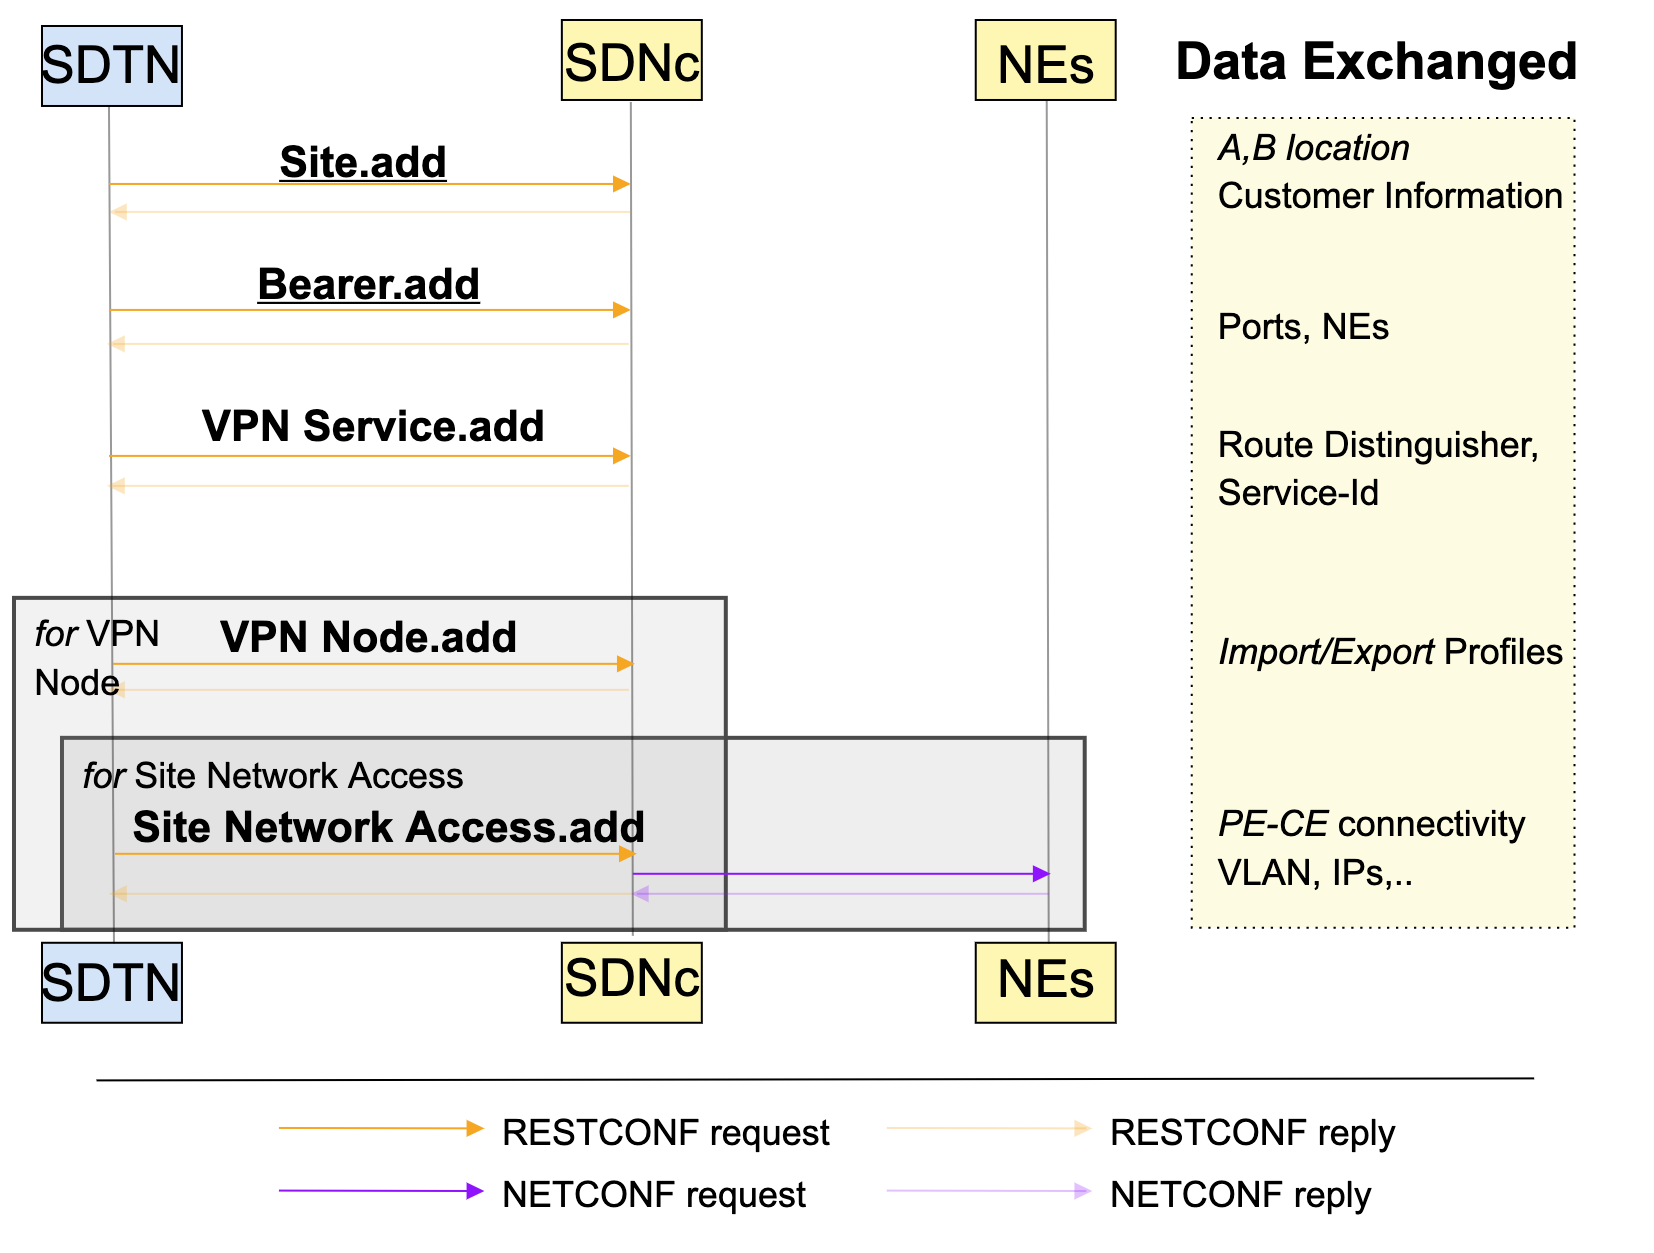
\includegraphics[width=\linewidth]{figs/diagram-9.png}
	\caption{Messages Interchange for IP multi-domain L3VPN service creation.}
	\label{FIG:l3vpn_workflow}
\end{figure}

The parameters delegation done by the SDTN \added{Controller} had the following four steps per domain.
\begin{enumerate}
    \item Create Site: Indicates the place where the services end-points are located. It unclude magement information and service descriptions. 
    \item Create Bearer: Indicates the NE and the Port assigned to the service.
    \item Create VPN-Node: Indicates the VRF deployment and all its attributes on the PE. It includes the import/export policies.
    \item Create Site Network Access: Refers to the CE-PE connectivity attributes. Such as routing protocol exchanged, IP addressing or ethernet encapsulation. 
\end{enumerate}

\Cref{FIG:l3vpn_workflow} depicts the corresponding workflow to create the L3VPN. Each step in the figure matches the sequence previously described. A similar workflow was used for all the RESTCONF operations like Create, Read, Update and Delete. 

\section{Field Trial Environment for i\uppercase{FUSION} SDTN Demonstration}
\label{section:trial}

In this work, we have deployed the i\uppercase{Fusion} architecture in a Telefonica Colombia field trial environment. The field trial includes not just the i\uppercase{FUSION} SDN control layer (\Cref{sec:contollay}), but also the network elements described in \Cref{sec:netlay}.

\subsection{SDN Control Layer}
\label{sec:contollay}
The SDN control layer architecture was built upon the reference design guidelines described in \Cref{section:arq}. The key elements of the control layer was:
\begin{itemize}
    \item Infinera Trascend Maestro, acting as SDTN controller.
    \item 2 x IP SDNcs one for each IP domain. 
    \item 2 x Optical SDNcs one for each optical domain.
\end{itemize}

SDNcs communicate with NEs via NETCONF/YANG and RESTCONF/YANG with SDTN \added{Controller} using the Data Communication Network (DCN). The optical and IP SDNcs are commercial products from the network element vendors.  

\subsection{Network Elements}
\label{sec:netlay}
The set-up for this field trial uses a full network with all the Hierarchical Levels (HL) that compose a Service Provider real environment. In our notation and architecture the IP/MPLS-based network is comprised of five (5) HLs with the following responsibilities: 

\begin{itemize}
    \item HL1: Core PE-Routers acts as Toll Gates for the Service Provider's interconnection with other carriers and using eBGP logical structure for publishing public IPv4/IPv6 prefixes. 
    \item HL2: Core P-Router is responsible for the transportation of traffic between main cities and metropolitan areas sending/receiving traffic to HL1 interconnections from/to the International Internet. Two (2) vendor B routers were used as HL2. The core routers run in an isolated IGP domain.
    \item HL3: PE-Routers are responsible for the aggregation of traffic from metropolitan and regional areas for both fixed and mobile services. Moreover, some HL3s provide connectivity to 4G/5G platforms (EPC, packet core, etc.).
    Four (4) routers were used as HL3s, distributed in two IGP domains (two for each vendor).
    \item HL4s collect traffic from fixed access networks (DSLAM/CMTS/OLT) in metropolitan areas and high capacity corporate services. Five (5) routers were used HL4 devices: three (3) for vendor A and (2) for vendor B. Each PE has connectivity to the both HL3 routers of its island.
    \item HL5: Cell Site Routers connects corporations, enterprises, small businesses and mobile terminal nodes (BTS, NodeB, eNodeB) in remote areas. Formerly known as cell site routers in Mobile Service Providers, but they evolved and converged to serve multiple fixed plus mobile segments. One HL5 was used in these tests from vendor A.
\end{itemize}

The IP/MPLS network was build using seamless MPLS option-C. Clusters and rings organized the network—IP clusters groups devices of a specific vendor. As a seamless MPLS, the underlay signaling requires that every origin PE-Routers (HL4) from a cluster can establish an end-to-end path to the destination PE-Router (HL4) even if the destination belongs to a different cluster. 

Thus, the HL3 routers from each region establish an eBGP session against the Core-Routers (HL2). This session exports the Router-ID plus Label information of all the routers in the region using BGP label unicast (LU). Additionally, another eBGP session between the HL3 of the region and the core Router-Reflectors to export the VPNv4 routes from each VPN service. This eBGP session requires a mandatory Next-Hop-Unchanged configuration to avoid network loops or misconfigured paths. 

Two-vendor WDM infrastructures transported the IP/MPLS links of vendor B HL2s and vendor A HL3s. The optical transport infrastructure was built as two independent metropolitan optical networks. We used (4) four nodes in each optical network with 100Gb and 10Gb lambdas for these experiments. 

\subsection{Multi-domain IP L3VPN provisioning}

This section presents the test results for the Hierarchical SDTN Controller integration with the controllers in the IP/Optical domains. Two types of tests have been done to demonstrate orchestration functionalities in the multi-layer/multi-domain/multi-vendor network environment, as depicted in \Cref{FIG:testing_workflow}. In a first stage, each \replaced{SDNc}{SDN controller} was validated individually. RESTCONF-based queries were sent towards each of the SDNCs to change and retrieve the network information and validate each implementation's compliance. This initial certification aimed to make functional tests over each solution and speed-up the entire solution's final integration. The scalability and efficiency of the SDTN \added{Controller} solution is limited to the SDNc performance.

\begin{figure}
	\centering
		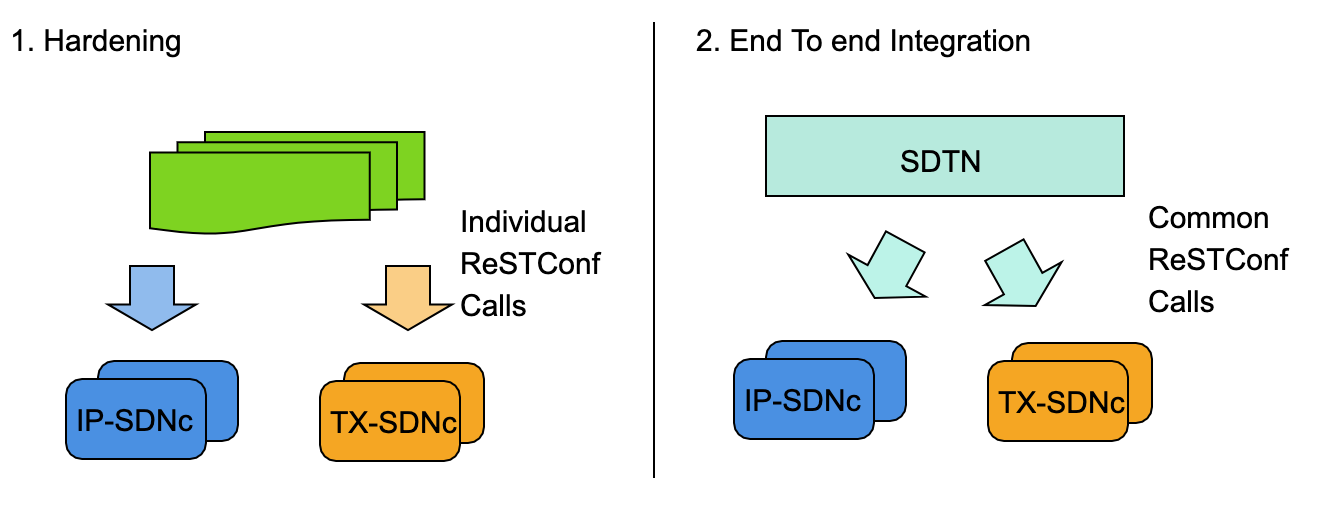
\includegraphics[width=\linewidth]{figs/diagram-11.png}
	\caption{The two types of tests have been done in order to demonstrate orchestration functionalities in the multi-layer/multi-domain/multi-vendor network environment. (1) Hardening process includes single domain tests. (2) End to end integration includes the SDTN \added{Controller} delegation of resources to the domain controllers.}
	\label{FIG:testing_workflow}
\end{figure}

\begin{figure*}
	\centering
		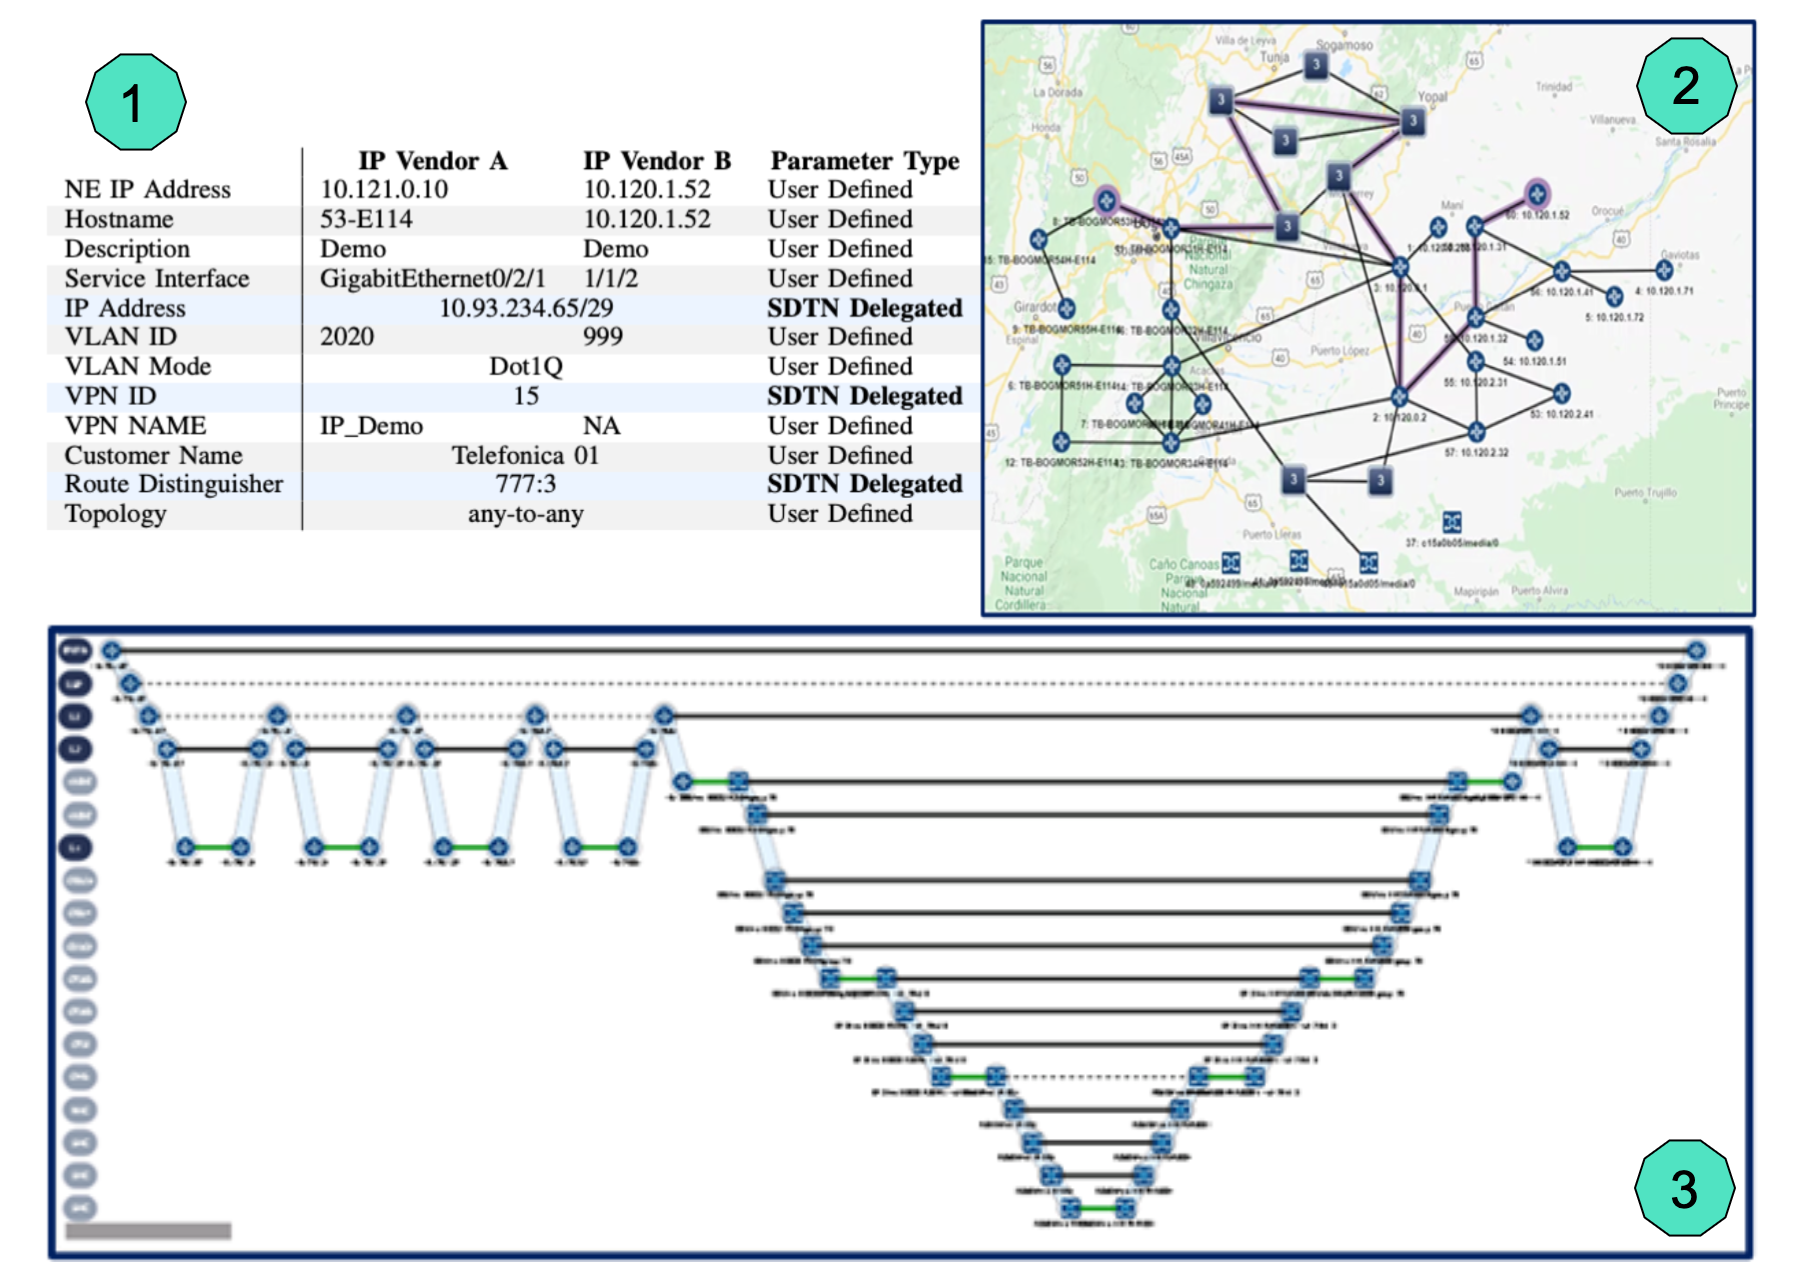
\includegraphics[width=\linewidth]{figs/diagram-14.png}
	\caption{L3VPN service creation results retrieved from the SDTN \added{Controller} GUI. Included three visualization panes: The service details (Name, Topology, RD and Endpoints), the geographical view and the hop-by-hop connection view.}
	\label{FIG:l3vpn_results}
\end{figure*}


Once each domain controller was independently certified during the individual validation process, the end-to-end integration was done using multi-domain functional tests. In that case, the Transcend Meastro GUI was used to orchestrate the entire service lifecycle. For example,  to create a service between two domains, the SDTN \added{Controller} provided a Graphical template to fill the service creation parameters. The parameters depicted in \Cref{FIG:l3vpn_results} includes the user-defined configuration requirements and the auto-assigned parameters by the SDTN \added{Controller}. In both cases, the SDTN \added{Controller} stored the whole service resources, and It continuously monitors the network state to keep the set of values synchronized. The workflow used is by the SDTN is depicted in \Cref{FIG:l3vpn_workflow}. Each time a user created a service, a set of request calls was instantiated between the SDTN \added{Controller} and the corresponding SDNc. Finally, once the SDNc confirms the service creation to the SDTN \added{Controller}, the Transcend Maestro provided three visualization options: (1) Service details, (2) Geographical view, and (3) Layered view, as depicted in \Cref{FIG:l3vpn_results}.

\begin{enumerate}
    \item The VPN service details including the service name, the topology and end-points. 
    \item The service route in the topology view, this view includes the full path including the IP and Optical devices compromised in the service.
    \item Layered view of the service. This view splits the service connections between layers, so the IP Links connection is in the top. The Ethernet connections between routers are in the second layer and physical plus optical layers are decoupled in this hierarchical structure.
\end{enumerate}

\begin{figure*}
	\centering
		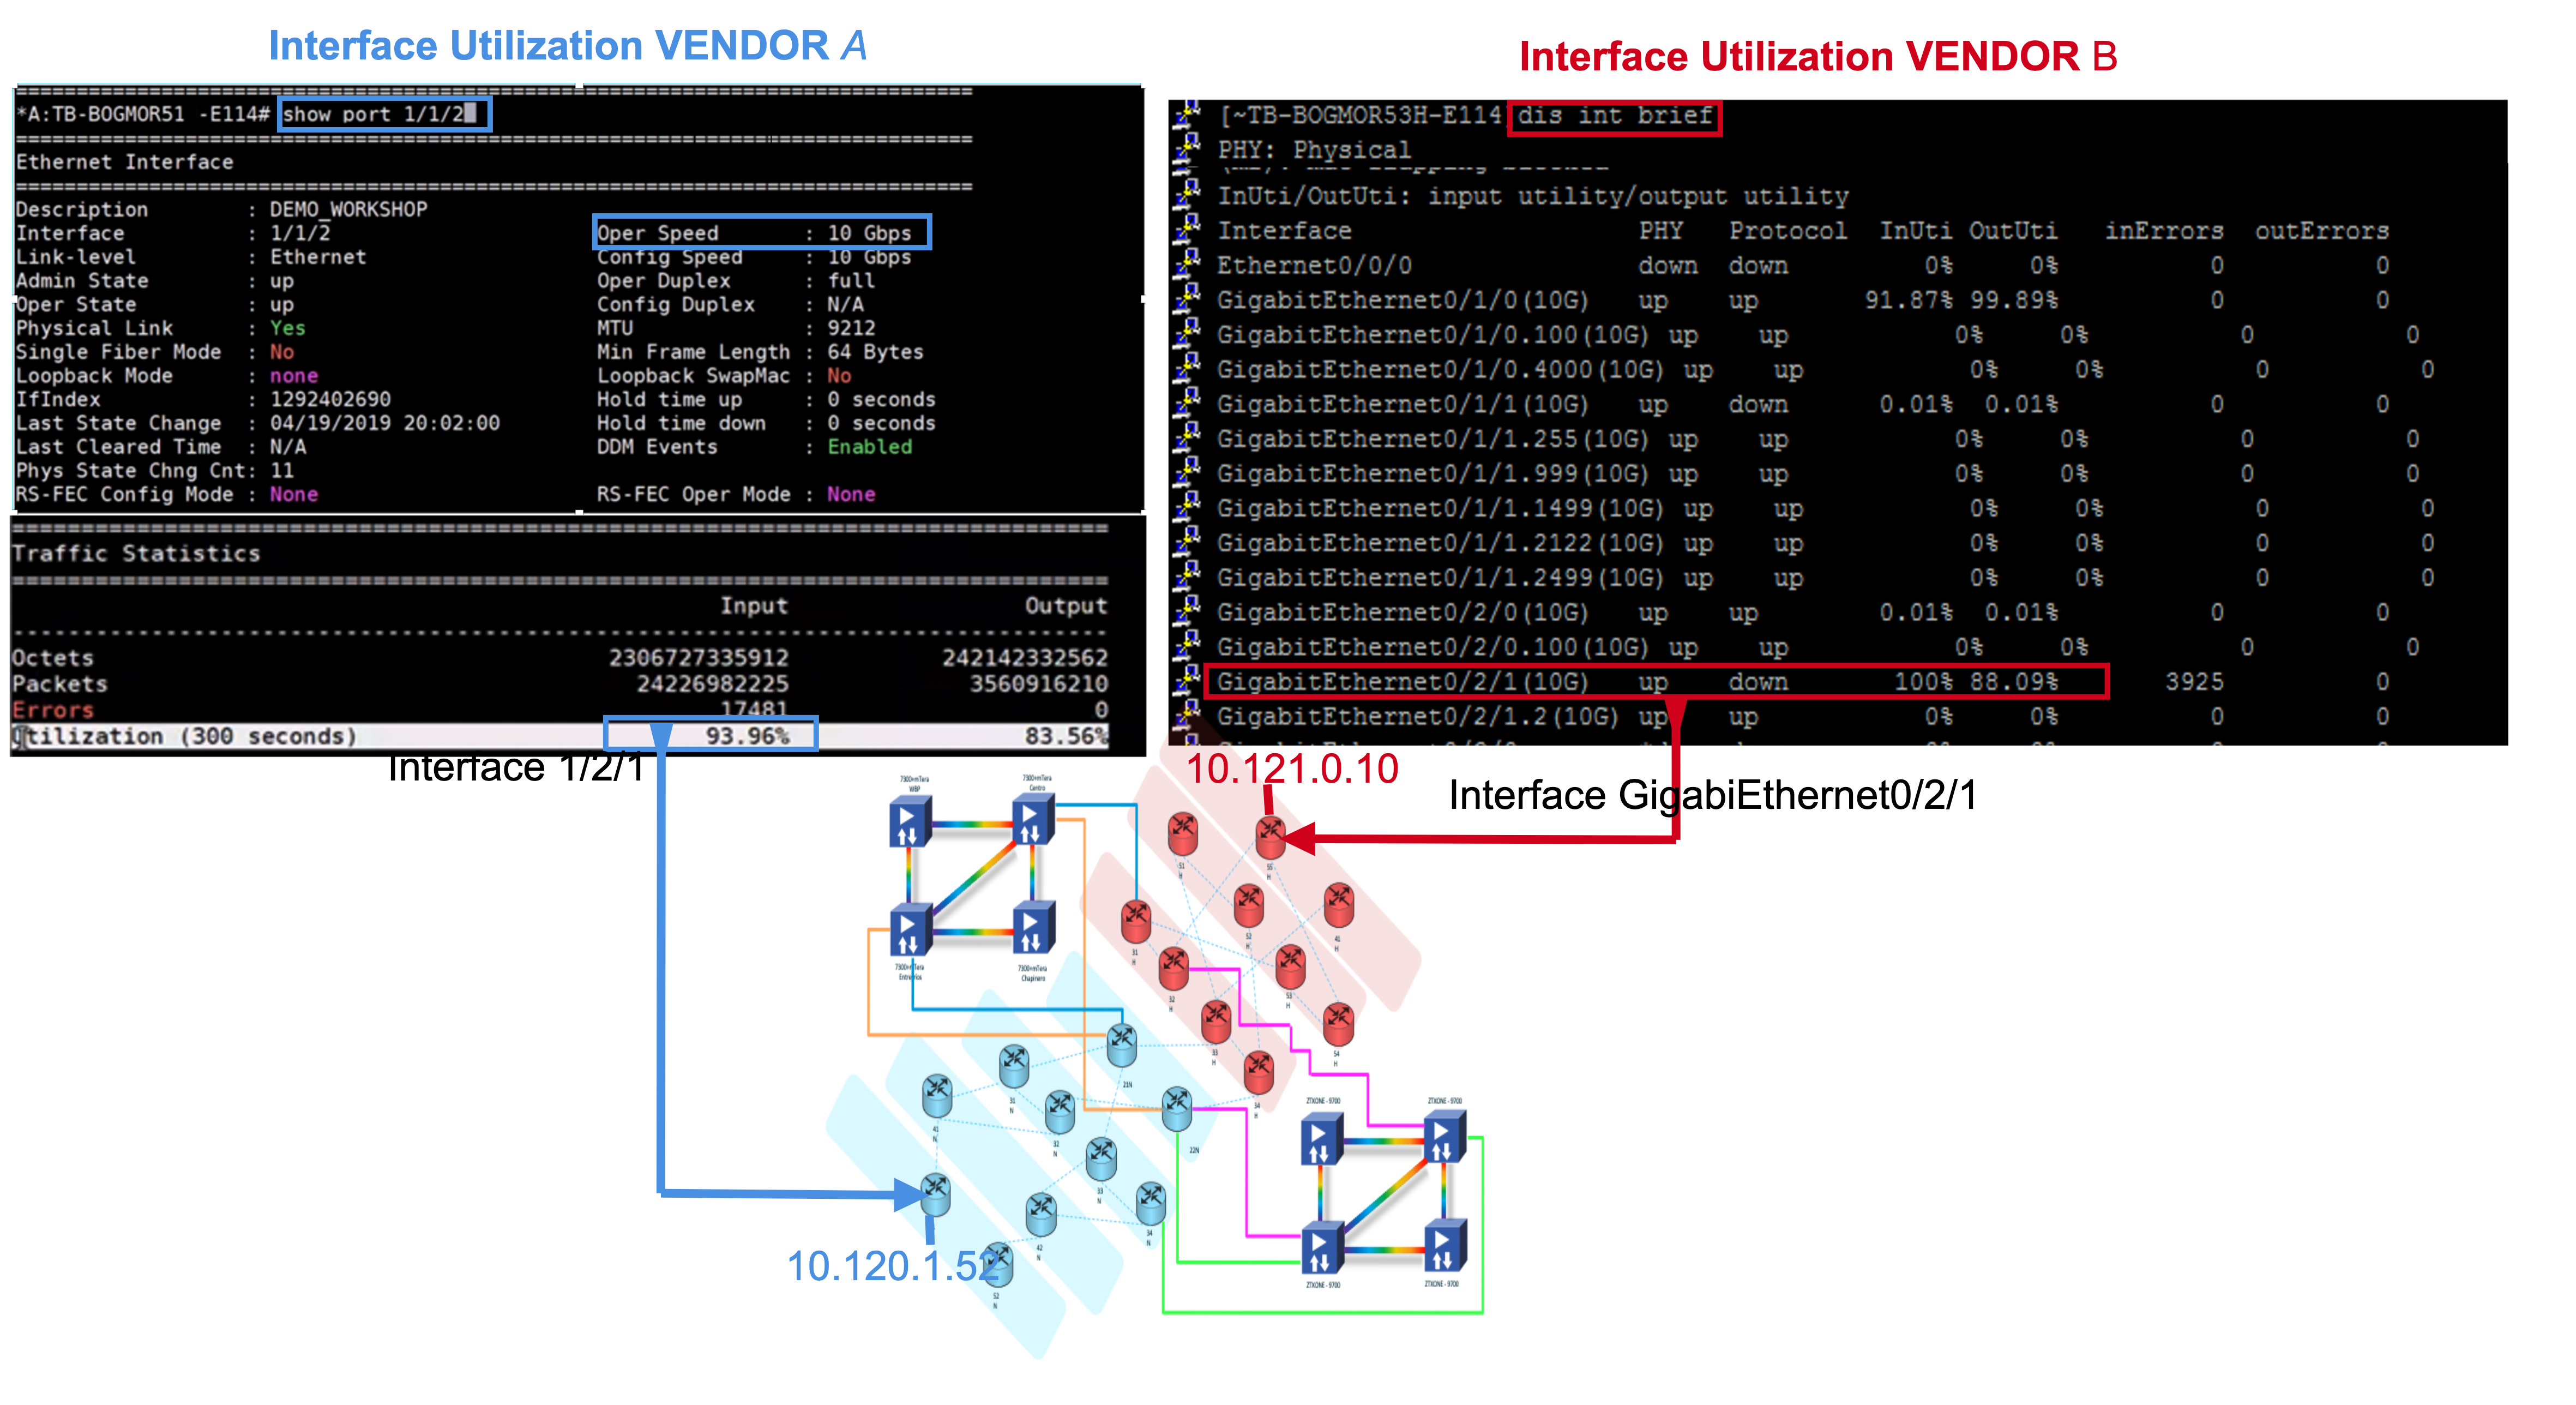
\includegraphics[width=\linewidth]{figs/counters1.png}
	\caption{Traffic counters measured on the end-points of the service. The utilization in both ends is close to 95\% due to the traffic injected by the generator.}
	\label{FIG:counters}
\end{figure*}


The configuration of the IP L3VPN service in the network elements was verified by using their command line interface as well as the IP\replaced{SDNc}{-SDN controllers} GUI. To validate the data plane, a traffic generator was used in site to introduce traffic on both ends of the network and tested the multi-domain L3VPN service. \Cref{FIG:counters} shows the traffic statistics as seen on the command-line interface of the PE routers. In this figure, the two interfaces connected to the VPN services are selected, and their traffic counters are showed. \replaced{Figure 6 shows the bandwidth utilization of 93.96\% and 88\% on each end of the VPN service.}{The occupancy of the 10G ports is close to the 95\% during the test.} 

\section{Conclusions and Future Work}
\label{section:conclusions}
 
\replaced{It is fundamental for the SDN adoption in service provider networks defining the data models and protocols used across the components.}{A key angular stone for the SDN adoption in service provider networks is the definition of the data models and protocols to be used by the architecture components for the integration between them.} Historically, integration using proprietary interfaces delay the introduction of programmability and automation and have a high economic cost. In this work, RESTCONF with IETF YANG models was tested for the integration between the SDTN \added{Controller} and the IP SDNcs. \added{This work shows, for the first time,} a standardized \added{L3NM} API to provision and retrieve services to a multi-vendor underlay network. \added{Moreover, this paper presents an infrastructure using network elements in the production network of Telefonica Colombia.}

The tests included the provision of L3VPN using IETF YANG data models and the topology collection. The SDTN \added{Controller} orchestrated the service creation assigning the resources to each domain controller. During the service retrieval, the SDTN \added{Controller} composed the services based on the information exposed by the domain controllers.

For additional tasks, there are still gaps to cover all the IP/MPLS network operation requirements. A brief summary of the issues faced during the integration, as reference point to future work are: 

\begin{itemize}
    \item Connectivity, latency and internal processing times between the HCO and some of the SDNcs can impact the integration and result in miscommunications creaking the timeout of SDN transport protocols, ie. RESTCONF and NETCONF.   
    \item \textit{Ghost} objects which would not be completely deleted in the controllers can lead to misunderstand in the topology construction.
    \item The unsolicited data retrieved by a lack of standardization or a bias in the implementation of the standards can lead to uncompleted transactions or loops in execution tasks.
    \item Absence of data in the SDN domain controllers for an automatic inter-domain link discovery.
    \item Differences in the RESTCONF/YANG implementations on the \replaced{SDNc}{SDN Controllers}. Even if the YANG models were the same, the parameters translation between NBI and SBI can restrict some configurable parameters (i.e max length size of a description field) and may generate implementation differences. This would derive in possible errors during the execution of the creation process.
    \item Differences in the RESTCONF/YANG error handling. A set of well defined error codes is mandatory in the hierarchical architecture.
\end{itemize}

The APIs designed in this work demonstrates the viability of the i\uppercase{FUSION} architecture with an SDTN \added{Controller} orchestrating an underlay multi-vendor, multi-layer, and multi-domain network environment. The i\uppercase{FUSION} APIs allow any service provider to migrate brownfield scenarios into SDN-ready domains using programmatic interfaces.

\subsection{Future Work}
As future work, the hybrid SDN deployment done until now must be complemented with an integration between the NBI exposed by the SDTN \added{Controller} and the OSS applications ecosystem. The OSS ecosystem can include for example strategic and tactical planning applications, able to support the year by year demand management and planning tasks done within the organization. A common interface defined and available for these tasks would allow the OSS systems providers to focus on the quality of the applications developed, forgetting the complexity of the network management. Economically it will generate direct reductions in the applications integration time.

\section*{Acknowledgements}
This \deleted{is} work has been supported by Telefonica I+D as part of the Fusion, i\uppercase{FUSION}, OpenFusion projects and partially funded by the EC 5GPPP TeraFlow (101015857) and MINECO AURORAS (RTI2018-099178-B-I00). Authors would like to thank to all the SDN technical teams and leaders that participate in the development, deployment, and testing of this \deleted{SDTN} architecture. Many thanks for their contributions to Manuel Santiago, Gloria Gomez, Julia Rodriguez and Zdravko Stevkovski from Infinera, Randy Quimbay, David Rocha from Telefonica Colombia, and Andrea Valencia, Juan Suarez, Juan Agredo and Daniel Hernandez from Wipro.   

\bibliographystyle{IEEEtran}
\bibliography{Biblio}

\begin{IEEEbiography}
[{
\includegraphics[width=1in,height=1.25in,clip,keepaspectratio]{figs/Bio/1010179793S.jpg}}]%
{Samier Barguil} (M.Sc. 2018). PhD Candidate from the Universidad Autonoma de Madrid. Electronic Engineer from the District University of Bogot\'a Franscisco José de Caldas and Master in Science in Industrial Automation of the Universidad Nacional de Colombia. Currently is the IP SDN Technical Leader at Wipro Technologies Ltd.\end{IEEEbiography}

\begin{IEEEbiography}[{
\includegraphics[width=1in,height=1.25in,clip,keepaspectratio]{figs/Bio/victor.jpg}}]%
{Víctor López} (M.Sc. 2005 - Ph.D. 2009) is a Technology Expert at Systems and Network Global Direction in Telefónica gCTIO. He works on the global IP and transport processes of the Telefonica group. He serves as co-chair at the Open Optical Packet Transport group in the Telecom Infra Project. He has co-authored more than 200 publications, six patents and contributed to IETF and ONF. Moreover, he is the editor of the book Elastic Optical Networks: Architectures, Technologies, and Control. His research interests include the integration of Internet services over IP/MPLS and optical networks and control plane technologies (PCE, SDN, GMPLS).\end{IEEEbiography}

\begin{IEEEbiography}[{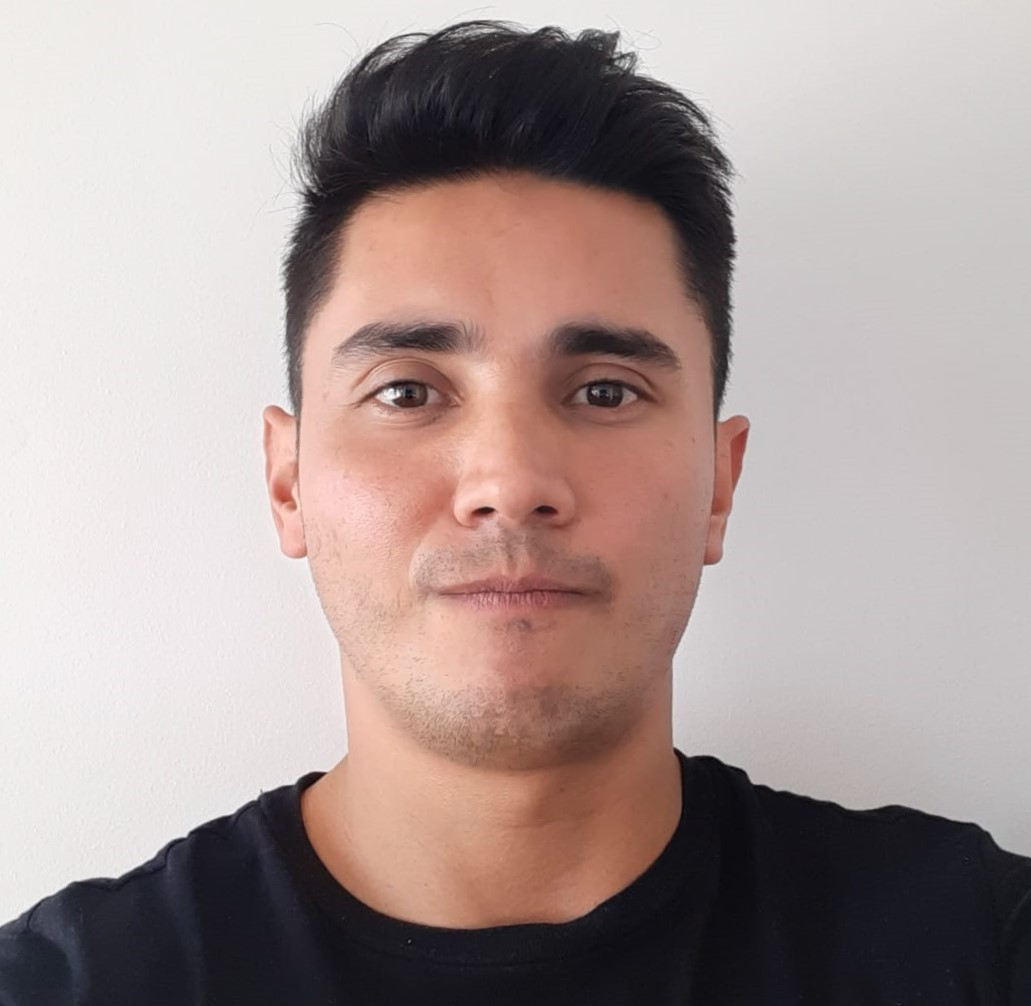
\includegraphics[width=1in,height=1.25in,clip,keepaspectratio]{figs/Bio/cristyan_manta.jpeg}}]%
{Cristyan Manta-Caro} (M.Sc. 2007 - PhD (c)) currently serves as Solutions Manager and Managing Consultant at Wipro Technologies Ltd within the Comms EGM BU. He is responsible for structuring and leading transformation projects for Digital and Telecommunications providers. With over 15 years of experience in managing, optimizing, analyzing telecommunications and Information Technology IT infrastructures with primary vendors and CSP. His research interests include SDN architectures, Future Internet, DevNet \& NetDevOps, Cloud Technologies for IoT and the Web of Things WoT.\end{IEEEbiography}

\begin{IEEEbiography}[{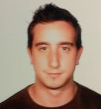
\includegraphics[width=1in,height=1.25in,clip,keepaspectratio]{figs/Bio/arturomayoral.png}}]%
{Arturo Mayoral López de Lerma} is a Technology Expert in Transport Networks at the Global Systems \& Network department of Telefónica GCTIO. He received the Ph.D. degree in telecommunications engineering from the Universitat Politècnica de Catalunya (UPC) in 2019. His  research  interests  include  optical network design and Software Defined Networking (SDN). He graduated in Telecommunications Engineering by the Universidad Autónoma de Madrid in 2013 and he started his professional career in 2012, as undergraduate researcher in Telefonica I+D (R\&D) where developed his Final Career’s Project, awarded with the Best Final Project Prize by the Official College of Telecommunication Engineers (COIT).\end{IEEEbiography}

\begin{IEEEbiography}[{
\includegraphics[width=1in,height=1.25in,clip,keepaspectratio]{figs/Bio/ogondio.png}}]%
{Oscar González de Dios} received his M.S. degree in telecommunications engineering and Ph.D. degree (Hons.) from the University of Valladolid, Spain. He has 19 years of experience in Telefonica I+D, where he has been involved in a number of European research and development projects (recently, STRONGEST, ONE, IDEALIST, and Metro-Haul). He has coauthored over 100 research papers and 10 IETF RFCs. He is currently the head of SDN Deployments for Transport Networks, Telefonica Global CTIO. His main research interests include photonic networks, flexi-grid, interdomain routing, PCE, automatic network configuration, end-to-end MPLS, performance of transport protocols, and SDN. \end{IEEEbiography}

\begin{IEEEbiography}[{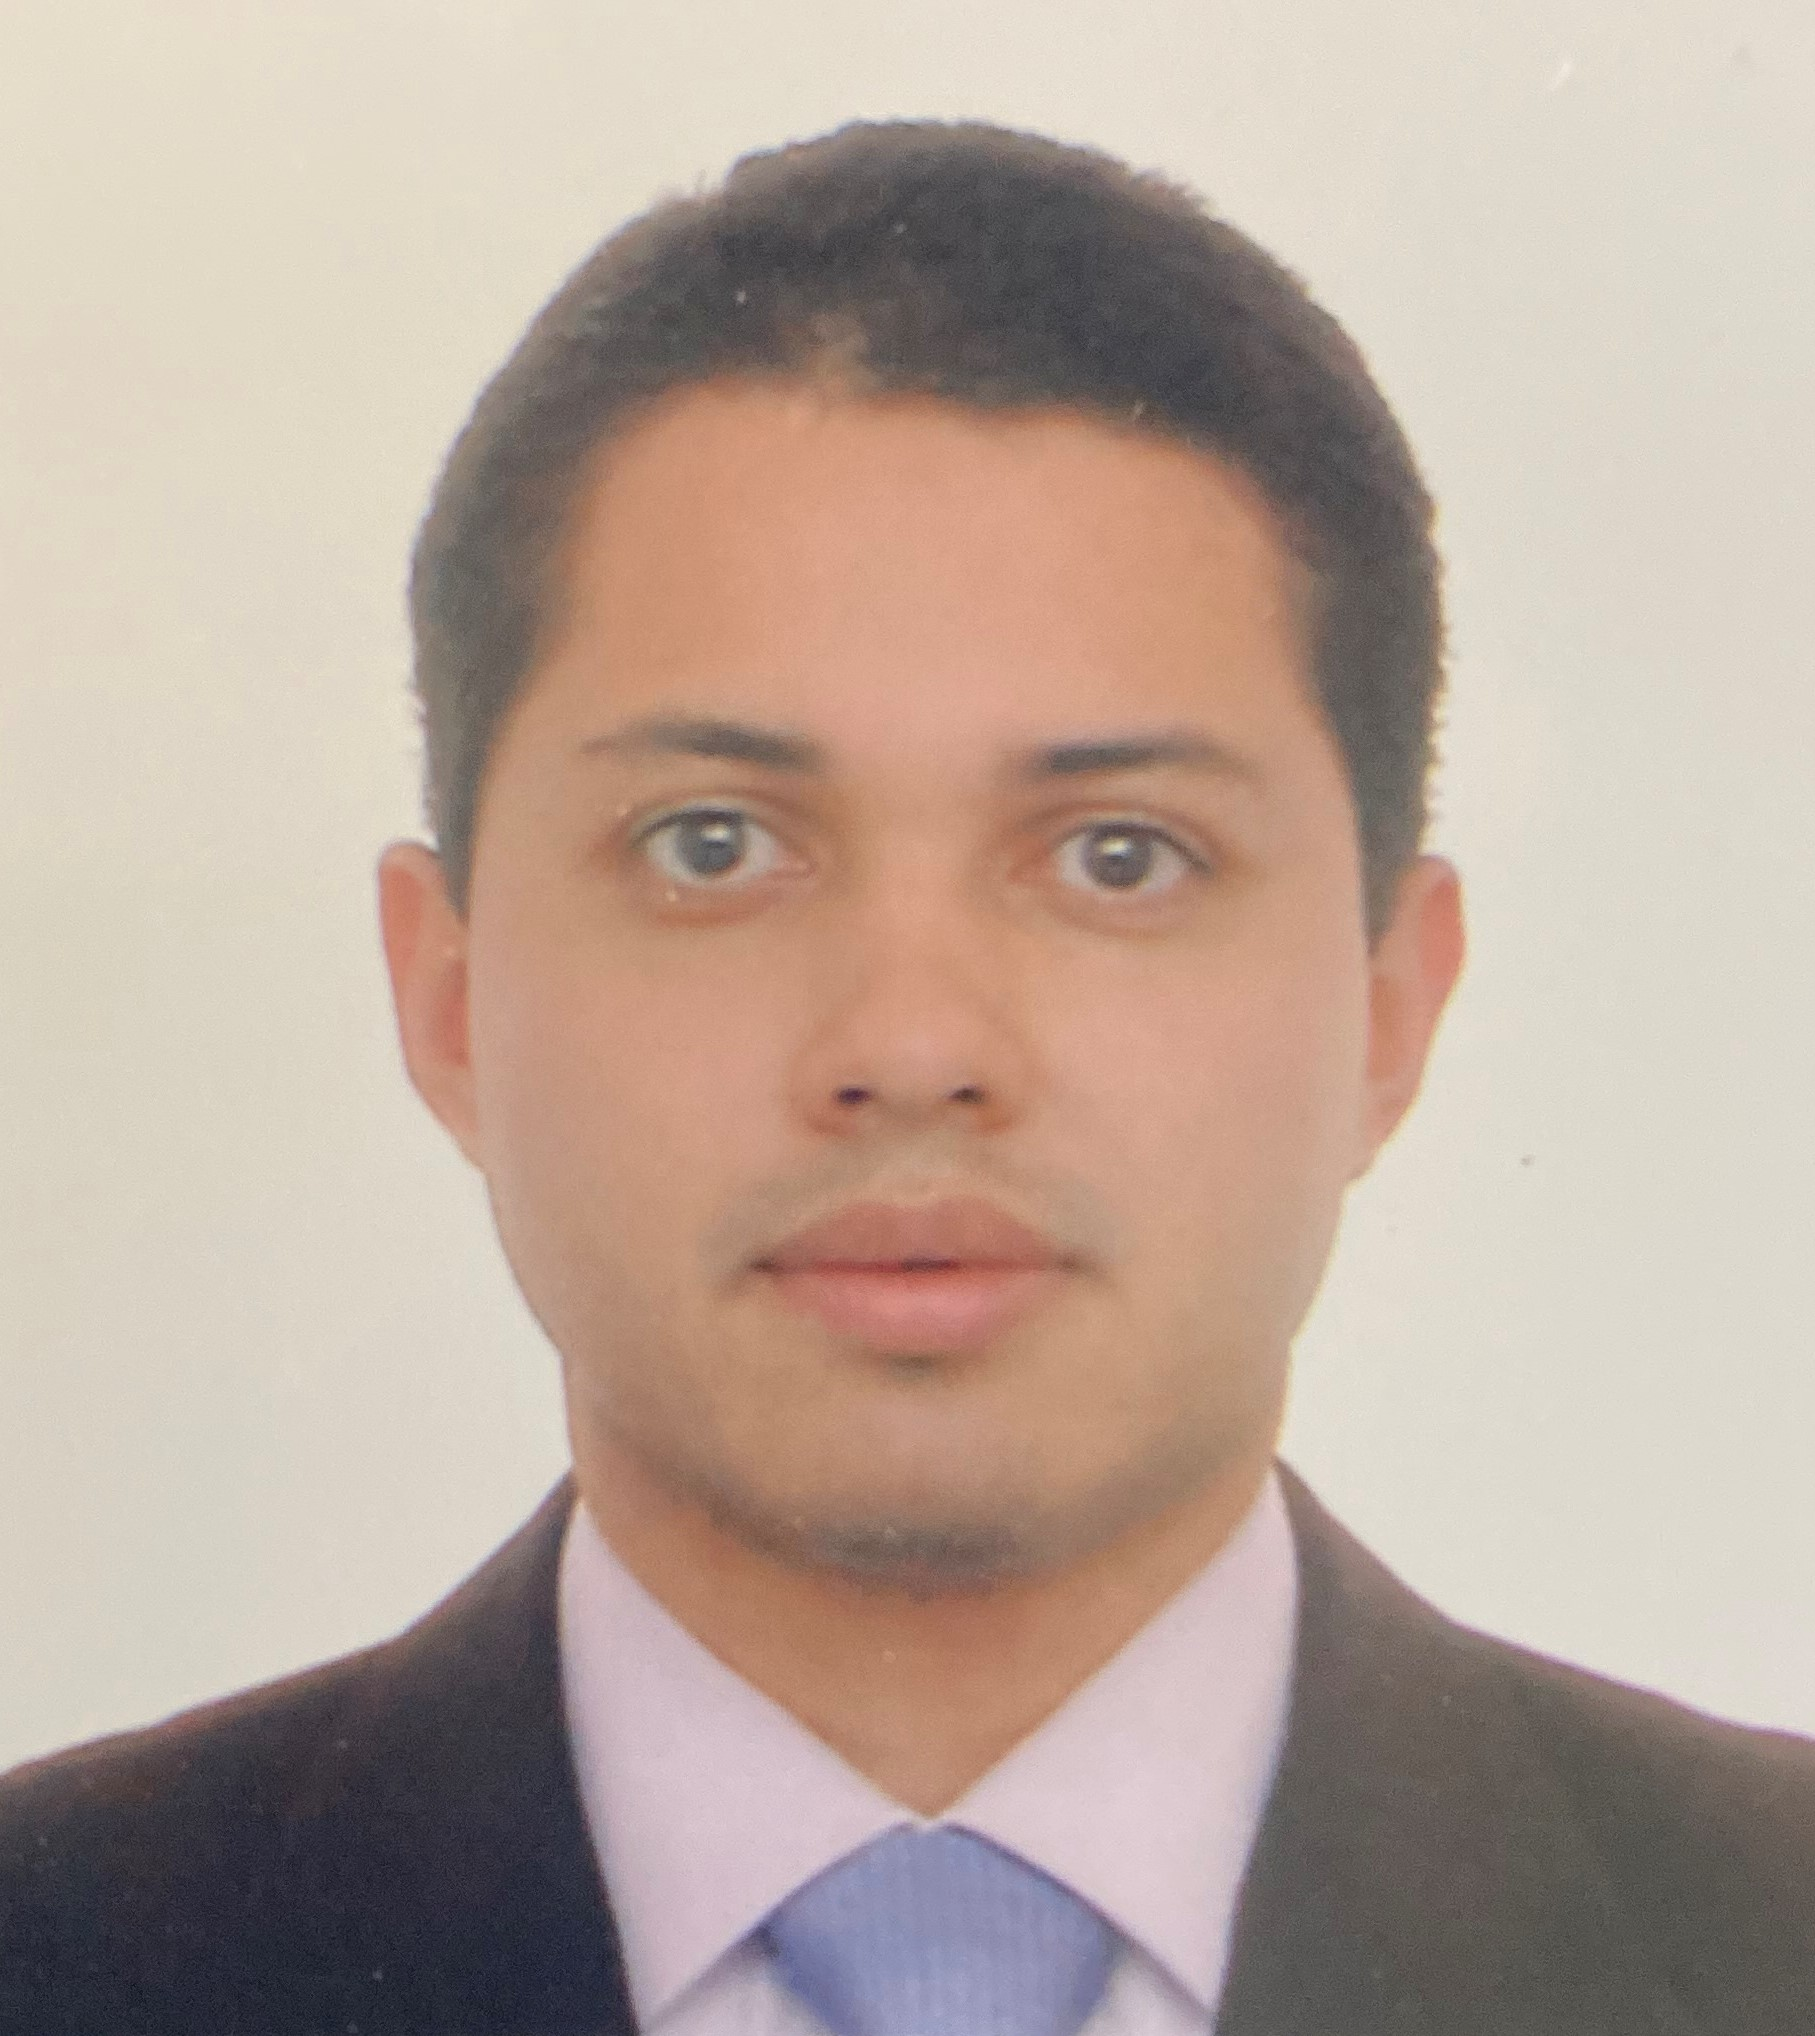
\includegraphics[width=1in,height=1.25in,clip,keepaspectratio]{figs/Bio/Edward_Echeverry.jpg}}]%
{Edward Echeverry} is Head Of Transport (IP and Optical Network) in Telefonica Colombia. Electronic Engineer, Telecommunications Specialist with a 15+ years of experience in the field. High technical skills and advanced experience in the design, planning and implementation of 3G/4G mobile, IP/MPLS and new generation optical networks, as well as in management and deployment of projects. architectures.\end{IEEEbiography}

\begin{IEEEbiography}[{
\includegraphics[width=1in,height=1.25in,clip,keepaspectratio]{figs/Bio/juan_pedro.png}}]%
{Juan Pedro Fernández-Palacios Giménez} received the MS in Telecommunications Engineering from Polytechnic University of Valencia in 2000. In Sept. of 2000 he joined Telefonica I+D where his research activities where focused on the design of new data and control plane architectures for IP over optical networks. He is author of 6 patents filled in Europe and US and more than 70 publications in conferences and journals. He was coordinator of two European research projects on optical transport networks (MAINS and IDEALIST). Since June 2017 he is leading the Integrated Transport Centre, a global organization in Telefonica in charge of defining the strategic network planning and technology for IP, DWDM, MW and satellite. networks.\end{IEEEbiography}

\begin{IEEEbiography}[{
\includegraphics[width=1in,height=1.25in,clip,keepaspectratio]{figs/Bio/janne_karvonen_640x640.jpg}}]%
{Janne Karvonen} (M.Sc.(Tech.) 1993 Helsinki University of Technology) is a Senior Software Architect at Infinera Corporation. He works in the Systems Architecture Group, focusing on Software Defined Networking Technologies and IP/MPLS Network Management Systems. He has over 30 years of experience in Software Engineering and more than 20 years of experience in Telecommunications Network Management Systems, covering both optical and packet based technologies. His research interests include SDN technologies for multi-layer, multi-domain and multi-vendor networks, with special focus on SDN API technologies, Multi-Layer Path Computation Algorithms and utilization of Machine Learning in SDN networks.\end{IEEEbiography}

\begin{IEEEbiography}[{
\includegraphics[width=1in,height=1.25in,clip,keepaspectratio]{figs/Bio/jutta_685x685.jpg}}]%
{Jutta Kemppainen} received her Master of Science (Tech.) in 1999 from Helsinki University of Technology (now part of Aalto University). She works as Senior Principal Product Manager at Infinera, managing Infinera multi-layer, multi-domain and multi-vendor transport network automation solutions. She has over 20 years of experience of telecommunications software automation products and has been concentrating on Software-Defined Networking (SDN)-based solutions in the last 7+ years. During this time Kemppainen has been co-operating with 70+ network providers, including many of the largest and technically most advanced in the industry, in designing and defining requirements for practical transport network automation solutions.\end{IEEEbiography}

\begin{IEEEbiography}[{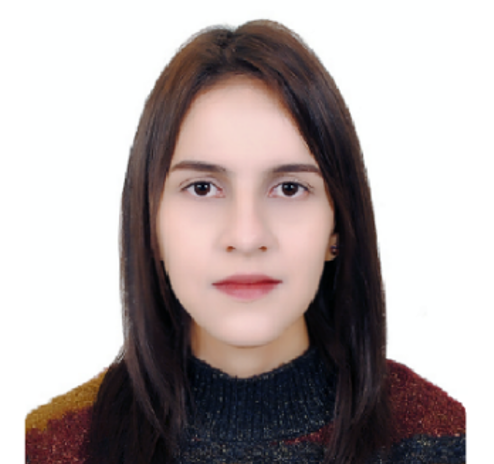
\includegraphics[width=1in,height=1.25in,clip,keepaspectratio]{figs/Bio/natalia_maya.jpg}}]%
{Natalia Isabel Maya Perfetti} is an Electronics and Telecommunications engineer graduated from Universidad del Cauca, Colombia back in 2018; thence, she has been working as a network planning engineer in Infinera Colombia where she supports different tasks related to DWDM Network Planning. For the last year she has also been responsible for the testing of the SDTN solution in the field trial environment.\end{IEEEbiography}

\begin{IEEEbiography}[{
\includegraphics[width=1in,height=1.25in,clip,keepaspectratio]{figs/Bio/vilalta.jpg}}]%
{Ricard Vilalta} graduated in telecommunications engineering in 2007 and received a Ph.D. degree in telecommunications in 2013, both from the Universitat Politècnica de Catalunya (UPC), Spain. He joined CTTC in 2010, and he is a senior researcher in the Optical Networks and Systems Department. He is an active contributor in several standardization bodies such as ONF, ETSI, and IETF. He is also a member of the technical steering team of Open Transport Configuration \& Control in ONF. He is leading open source contributions and features in ETSI Open Source MANO with special focus on 5G technologies.\end{IEEEbiography}

\end{document}